\begin{name}
	{\tenchude}
	{\tendethi}
	{SỞ GDĐT HÀ TĨNH}
	{\thoigian}
\end{name}

\caulc
\Opensolutionfile{ans}[Ans/TT-THPT-SGD-HaTinh-NH24-25]
%   \Opensolutionfile{ansbook}[Ansbook/TT-THPT-SGD-HaTinh-NH24-25-TN]%---Nên đặt tên theo bài
  \setcounter{ex}{0}
 %%%==============Cau_EX1==============%%%
  \begin{ex}%[Dự án C đề thi thử THPT QG 2025]%[Đỗ Chí Tâm]%[2D1B1-1]
 	Hàm số nào dưới đây đồng biến trên khoảng $(-\infty ;+\infty)$?
 	\choice
 	{$y=-x^3-2x+1$}
 	{$y=\dfrac{x-2}{x+1}$}
 	{\True $y=3x^3+3x-2$}
 	{$y=2x^3-5x+1$}
 	\loigiai{
 		Xét hàm số $y=3x^3+3x-2$ có 
 		$y'=9x^2+3>0$, $\forall x \in \mathbb{R}$.\\
 		Vậy hàm số $y=3 x^3+3 x-2$ đồng biến trên $\mathbb{R}$.
 	}
 \end{ex}
 %%%==============End-Cau_EX1==============%%%
 %%%==============Cau_EX2==============%%%
 \begin{ex}%[Dự án C đề thi thử THPT QG 2025]%[Đỗ Chí Tâm]%[2D1B2-1]
 	Cho hàm số $y=f(x)$ có đạo hàm $f'(x)=\left(x^2-4\right)(x+2)(x-3)$ và liên tục trên $\mathbb{R}$. Số điểm cực trị của hàm số đã cho là
 	\choice
 	{$5$}
 	{\True $2$}
 	{$3$}
 	{$1$}
 	\loigiai{
 		Ta có: $f'(x)=0 \Leftrightarrow\left(x^2-4\right)(x+2)(x-3)=0\Leftrightarrow(x+2)^2(x-2)(x-3)=0 \Leftrightarrow\hoac{&x=-2 \\& x=2 \\& x=3.}$\\Với $x=-2$ là nghiệm kép.\\
 		Vậy hàm số đã cho có $2$ cực trị.}
 \end{ex}
  %%%==============End-Cau_EX2==============%%%
 %%%==============Cau_EX3==============%%%
 \begin{ex}%[Dự án C đề thi thử THPT QG 2025]%[Đỗ Chí Tâm]%[2D1Y3-1]
 	Cho hàm số $y=f(x)$ có bảng biến thiên như hình bên. Giá trị lớn nhất của hàm số đã cho trên đoạn $[-2;4]$ bằng
 	\begin{center}
 		
\begin{tikzpicture}[font=\normalsize,t style/.style={style=solid}]
 			\tkzTabInit[nocadre=true,lgt=1.2,espcl=2.5,deltacl=0.5]
 			{$x$ /0.75, $y'$/0.75, $y$/2}
 			{$ -\infty $,$ -1 $,$ 1 $,$ 3 $,$ +\infty $}
 			\tkzTabLine{,+,0,-,0,+,0,-, }  % z, t, d;
 			\tkzTabVar{-/$-\infty$,+/$10$,-/$-4$,+/$8$,-/$-\infty$} %+ hoac-
 		\end{tikzpicture}
 	\end{center}
 	\choice
 	{$-1$}
 	{\True $10$}
 	{$1$}
 	{$8$}
 	
 	\loigiai{
 		Từ bảng biến thiên, ta thấy giá trị lớn nhất của hàm số trên đoạn $[-2;4]$ là $10$.}
 \end{ex}
  %%%==============End-Cau_EX3==============%%%
 %%%==============Cau_EX4==============%%%
 \begin{ex}%[Dự án C đề thi thử THPT QG 2025]%[Đỗ Chí Tâm]%[2D1B5-3]
 	\immini{Cho hàm số đa thức bậc bốn $y=f(x)$ có đồ thị như hình vẽ bên. Phương trình $f(x)-1=0$ có bao nhiêu nghiệm thực phân biệt?
 	\choice
 	{\True $3$}
 	{$1$}
 	{$2$}
 	{$4$}}
 	{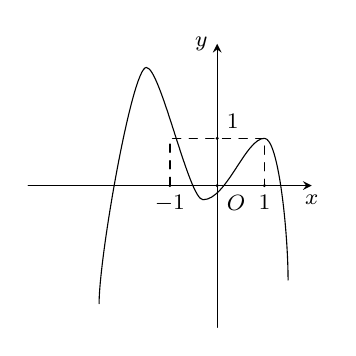
\begin{tikzpicture}[scale=0.6,>=stealth, font=\footnotesize, line join=round, line cap=round] 
 			\draw[->] (-4,0)--(2,0)node[below]{$x$};
 			\draw[->] (0,-3)--(0,3)node[left]{$y$};
 			\draw(-2.5,-2.5)..controls++(90:1) and++(180:0.3)..(-1.5,2.5)..controls++(0:0.3)and++(180:0.3)..(-0.3,-0.3)..controls++(0:0.5)and++(180:0.4)..(1,1)..controls++(0:0.3)and++(90:1)..(1.5,-2);
 			\draw(0,0)node[below right]{$O$};
 			\draw[dashed]
 			(-1,0)node[below]{$-1$}--(-1,1)--(0,1)node[above right]{$1$}--(1,1)--(1,0)node[below]{$1$};
 			\fill (0,0) circle (1pt);
 			\fill (0,1) circle (1pt);
 			\fill (-1,0) circle (1pt);
 			\fill (1,0) circle (1pt);
 		
 	\end{tikzpicture}}
 	\loigiai{
 		Ta thấy đường thẳng $y=1$ cắt đồ thị hàm số tại $3$ điểm phân biệt.
 		Do đó phương trình $f(x)-1=0$ có $3$ nghiệm phân biệt.}
 \end{ex}
  %%%==============End-Cau_EX4==============%%%
 %%%==============Cau_EX5==============%%%
 \begin{ex}%[Dự án C đề thi thử THPT QG 2025]%[Đỗ Chí Tâm]%[2D1B5-1]
 \immini{Đồ thị hàm số nào sau đây có hình dạng như hình vẽ?
 	\choice
 	{$y=x^3+3 x$}
 	{$y=x^3-3 x$}
 	{\True $y=x^3-3 x^2$}
 	{$y=x^3+3 x^2$}}
 	{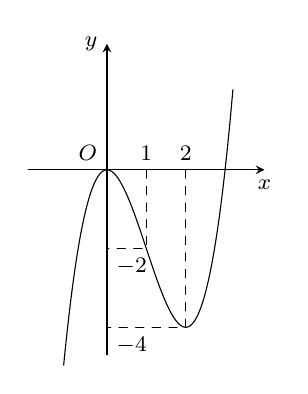
\begin{tikzpicture}[scale=0.5,>=stealth, font=\footnotesize, line join=round, line cap=round]
 			\draw[->] (-2,0)--(4,0)node[below]{$x$};
 			\draw[->] (0,-4.7)--(0,3.2)node[left]{$y$};
 			\draw[samples=100,domain=-1.1:3.2] plot (\x,{(\x)^3-3*(\x)^2});
 			\draw(0,0)node[above left]{$O$};
 			\draw[dashed]
 			(1,0)node[above]{$1$}--(1,-2)--(0,-2)node[below right]{$-2$}
 			(2,0)node[above]{$2$}--(2,-4)--(0,-4)node[below right]{$-4$};
 		\end{tikzpicture}}
 	\loigiai{
 		Ta thấy đồ thị hàm số đi qua điểm $(2;-4)$ nên đồ thị cho là đồ thị của hàm số $y=x^3-3x^2$.}
 \end{ex}
  %%%==============End-Cau_EX5==============%%%
 %%%==============Cau_EX6==============%%%
 \begin{ex}%[Dự án C đề thi thử THPT QG 2025]%[Đỗ Chí Tâm]%[1D6H4-3]
 	Tập nghiệm của bất phương trình $\left(\dfrac{1}{2}\right)^x<\dfrac{1}{8}$ là
 	\choice
 	{\True $(3;+\infty)$}
 	{$(-\infty; 3)$}
 	{$[3;+\infty)$}
 	{$(-\infty; 3]$}
 	\loigiai{
 		Ta có: $\left(\dfrac{1}{2}\right)^x<\dfrac{1}{8} \Leftrightarrow\left(\dfrac{1}{2}\right)^x<\left(\dfrac{1}{2}\right)^3 \Leftrightarrow x>3$.}
 \end{ex}
  %%%==============End-Cau_EX6==============%%%
 %%%==============Cau_EX7==============%%%
 \begin{ex}%[Dự án C đề thi thử THPT QG 2025]%[Đỗ Chí Tâm]%[2H3Y1-1]
 	Trong không gian $Oxyz$, cho $\overrightarrow{a}=2 \overrightarrow{i}-3
 	\overrightarrow{j}+\overrightarrow{k}$. Tọa độ của $\overrightarrow{a}$ là
 	\choice
 	{$(-2;1;3)$}
 	{\True $(2;-3;1)$}
 	{$(2;1;3)$}
 	{$(2;1;-3)$}
 	
 	\loigiai{
 		Ta có $\overrightarrow{a}=2 \overrightarrow{i}-3 \overrightarrow{j}+\overrightarrow{k}$. Suy ra 
 		tọa độ của vectơ $\overrightarrow{a}$ là $(2;-3;1)$.
 	}
 \end{ex}
  %%%==============End-Cau_EX7==============%%%
 %%%==============Cau_EX8==============%%%
 \begin{ex}%[Dự án C đề thi thử THPT QG 2025]%[Đỗ Chí Tâm]%[2H3Y1-1]
 	Trong không gian $Oxyz$, cho tam giác $ABC$ với $A(1;3;4)$, $B(2;-1;0)$, $C(3;1;2)$. Tọa độ trọng tâm $G$ của tam giác $ABC$ là
 	\choice
 	{$G\left(3;\dfrac{2}{3};3\right)$}
 	{$G(2;-1;2)$}
 	{\True $G(2;1;2)$}
 	{$G(6;3;6)$}
 	\loigiai{
 		Tọa độ trọng tâm $G$ của tam giác $ABC$ là $\heva{&x_G=\dfrac{x_A+x_B+x_C}{3}=2\\& y_G=\dfrac{y_A+y_B+y_C}{3}=1 \\& z_G=\dfrac{z_A+z_B+z_C}{3}=2.}$\\
 		Tọa độ trọng tâm $G$ của tam giác $ABC$ là $G(2;1;2)$.
 	}
 \end{ex}
  %%%==============End-Cau_EX8==============%%%
 %%%==============Cau_EX9==============%%%
 \begin{ex}%[Dự án C đề thi thử THPT QG 2025]%[Đỗ Chí Tâm]%[2H3B1-2]
 	Trong không gian $Oxyz$, cho $\overrightarrow{a}=(1;-2;2)$, $\overrightarrow{b}=(-1;2;1)$. Giá trị của tích vô hướng $\overrightarrow{a} \cdot \overrightarrow{b}$ bằng
 	\choice
 	{$3$}
 	{\True $-3$}
 	{$2$}
 	{$-2$}
 	\loigiai{
 		Ta có $\overrightarrow{a} \cdot \overrightarrow{b}=1 \cdot(-1)+(-2) \cdot 2+2 \cdot 1=-3$.
 	}
 \end{ex}
  %%%==============End-Cau_EX9==============%%%
 %%%==============Cau_EX10==============%%%
 \begin{ex}%[Dự án C đề thi thử THPT QG 2025]%[Đỗ Chí Tâm]%[1H8H6-1]
 	Cho hình chóp $S \cdot ABCD$ có $ABCD$ là hình vuông cạnh $a$, tam giác $SAD$ đều. Góc giữa hai đường thẳng $BC$ và $SA$ bằng
 	\choice
 	{\True $60^{\circ}$}
 	{$30^{\circ}$}
 	{$90^{\circ}$}
 	{$45^{\circ}$}
 	
 	\loigiai{
 		Vì  $AB\parallel BC \Rightarrow(SA,BC)=(SA,AD)=\widehat{SAD}=60^{\circ}$.
 	}
 \end{ex}
  %%%==============End-Cau_EX10==============%%%
 %%%==============Cau_EX11==============%%%
 \begin{ex}%[Dự án C đề thi thử THPT QG 2025]%[Đỗ Chí Tâm]%[1D5H2-2]
 	Trong tuần lễ bảo vệ môi trường, các học sinh khối $12$ tiến hành thu nhặt vỏ chai nhựa để tái chế. Nhà trường thống kê kết quả thu nhặt vỏ chai của học sinh khối $11$ ở bảng sau:
 \begin{center}
 		\begin{tabular}{|c|c|c|c|c|c|}
 		\hline Số vỏ chai nhựa & $[10{,}5;15{,}5]$ & $[15{,}5;20{,}5]$ & $[20{,}5;25{,}5]$ & $[25{,}5;30{,}5]$ & $[30{,}5;35{,}5]$ \\
 		\hline Số học sinh & $53$ & $82$ & $48$ & $39$ & $18$ \\
 		\hline
 	\end{tabular}
 \end{center}
 	Hãy tìm trung vị của mẫu số liệu ghép nhóm trên.
 	\choice
 	{$19{,}51$}
 	{\True $19{,}59$}
 	{$20{,}1$}
 	{$18{,}3$}
 	 	\loigiai{
 		Ta có $53+82+48+39+18=240$.\\
 		Như vậy nhóm $[15{,}5;20{,}5]$ chứa trung vị.\\
 		Khi đó $C=n_1=53$.\\
 		Trung vị của mẫu số liệu là $M_e=15{,}5+\dfrac{\dfrac{240}{2}-53}{82} \cdot(20{,}5-15{,}5) \approx 19{,}59$.
 	}
 \end{ex}
  %%%==============End-Cau_EX11==============%%%
 %%%==============Cau_EX12==============%%%
 \begin{ex}%[Dự án C đề thi thử THPT QG 2025]%[Đỗ Chí Tâm]%[2D1K4-1]
 \immini{Cho hàm số $y=\dfrac{ax^2+bx+c}{x}$ ($ac \neq 0$) có đồ thị hàm số như hình vẽ. Đường tiệm cận xiên của đồ thị hàm số đã cho là đường thẳng
 	\choice
 	{Đường thẳng $y=x$}
 	{\True Đường thẳng $y=-x$}
 	{Đường thẳng $x=0$}
 	{Đường thẳng $y=2x$}}
 	{\begin{tikzpicture}[scale=0.5,>=stealth, font=\footnotesize, line join=round, line cap=round]
 			\draw[->] (-6,0)--(6,0)node[below]{$x$};
 			\draw[->] (0,-6.5)--(0,6.5)node[right]{$y$};
 			\draw[samples=100,domain=-5:-0.7] plot (\x,{(-(\x)^2-4)/(\x)});
 			\draw[samples=100,domain=0.7:5] plot (\x,{(-(\x)^2-4)/(\x)});
 			\draw[samples=100,domain=-5:5] plot (\x,{-1*(\x)});
 			\draw(0,0)node[below right]{$O$};
 			\draw[dashed]
 			(-2,0)node[below]{$-2$}--(-2,4)--(0,4)node[right]{$4$}
 			(2,0)node[above]{$2$}--(2,-4)--(0,-4)node[left]{$-4$};
 			\end{tikzpicture}}
 	\loigiai{
 		Đồ thị hàm số đi qua các điểm $(2;-4)$, $(-2;4)$ nên $\heva{&\dfrac{4a+2b+c}{2}=-4 \\& \dfrac{4a- b+c}{-2}=4} \Leftrightarrow\hoac{&4a+2b+c=-8 \\& 4a-2b+c=-8.}$\\
 		Ta có $y=\dfrac{ax^2+bx+c}{x}=ax+b+\dfrac{c}{x} \Rightarrow y'=a-\dfrac{c}{x^2}$.\\
 		Mà $x=2$ là cực trị của hàm số nên $y'(2)=0 \Leftrightarrow a-\dfrac{c}{4}=0 \Leftrightarrow 4 a-c=0$.\\
 		Từ $(1)$ và $(2)$ suy ra $a=-1$, $b=0$, $c=-4$.\\
 		Vậy hàm số đã cho là $y=\dfrac{-x^2-4}{x}$\\
 		Vì tiệm cận xiên của đồ thị hàm số đi qua $O(0;0)$ nên nó có dạng $y=mx$ ($m \neq 0$).\\
 		Ta có $m=\lim\limits_{x \rightarrow+\infty} \dfrac{y}{x}=\lim \limits_{x \rightarrow+\infty} \dfrac{-x^2-4}{x^2}=-1$.\\
 		Vậy tiệm cận xiên của đồ thị hàm số là $y=-x$.
 	}
 \end{ex}
 %%%==============HetCau_EX12==============%%%
%  \Closesolutionfile{ans}
%  \Closesolutionfile{ansbook}
 
\cauds
%   \Opensolutionfile{ansbook}[Ansbook/TT-THPT-SGD-HaTinh-NH24-25-TF]%---Nên đặt tên theo bài
%   \setcounter{ex}{0}
 %%%==============Cau_EX1==============%%%
 \begin{ex}%[Dự án C đề thi thử THPT QG 2025]%[Đỗ Chí Tâm]%[2D1K3-6]
 	Một loại thuốc được dùng cho một bệnh nhân và nồng độ thuốc trong máu của bệnh nhân được giám sát bởi bác sĩ. Biết rằng nồng độ thuốc trong máu của bệnh nhân sau khi tiêm vào cơ thể trong $t$ giờ được cho bởi công thức $c(t)=\dfrac{t}{t^2+1}$ (mg/l).
 	\choiceTF
 	{\True  Sau khi tiêm thuốc $2$ giờ thì nồng độ thuốc trong máu của bệnh nhân bằng $0{,}4$ (mg/l)}
 	{Sau khi tiêm thuốc thì nồng độ thuốc trong máu của bệnh nhân có thể vượt quá $0{,}5$ (mg/l)} 
 	{\True Sau khi tiêm thuốc $1$ giờ thì nồng độ thuốc trong máu của bệnh nhân cao nhất}
 	{\True Sau khi tiêm thuốc thì nồng độ thuốc trong máu của bệnh nhân cao nhất bằng $0{,}5$ (mg/l)}
 	\loigiai{
 		\begin{itemchoice}
 			\itemch Sau khi tiêm thuốc $2$ giờ, nồng độ thuốc trong máu bệnh nhân là $c(2)=\dfrac{2}{2^2+1}=0{,}4$ (mg/l).\\
 			Ta có $c'(t)=\dfrac{t^2+1-2 t^2}{\left(t^2+1\right)^2}=\dfrac{1-t^2}{\left(t^2+1\right)^2}$
 			$$c'(t)=0 \Leftrightarrow 1-t^2=0 \Leftrightarrow\hoac{&t=1\, (\text{nhận})\\&t=-1\, (\text{loại}).}$$
 			Bảng biến thiên
 				\begin{center}
 				
\begin{tikzpicture}[font=\normalsize,t style/.style={style=solid}]
 					\tkzTabInit[nocadre=true,lgt=1.2,espcl=2.5,deltacl=0.5]
 					{$t$ /0.75, $c'(t)$/0.75, $c(t)$/2}
 					{$ 0$,$ 1 $,$ +\infty $}
 					\tkzTabLine{,+,0,-}  % z, t, d;
 					\tkzTabVar{-/$0$,+/$\tfrac{1}{2}$,-/$0$} %+ hoac-
 				\end{tikzpicture}
 			\end{center}
 			Từ bảng biến thiên ta thấy
 			\itemch Nồng độ thuốc trong máu không thể vượt quá $0{,}5$ (mg/l).
 			\itemch Sau khi tiêm thuốc $1$ giờ thì nồng độ thuốc trong máu bệnh nhân cao nhất.
 			\itemch Sau khi tiêm thuốc thì nồng độ thuốc trong máu của bệnh nhân cao nhất bằng $0{,}5$ (mg/l).
 		\end{itemchoice}	
 	}
 \end{ex}
 %%%==============HetCau_EX1==============%%%
  %%%==============Cau_EX2==============%%%
 \begin{ex}%[Dự án C đề thi thử THPT QG 2025]%[Đỗ Chí Tâm]%[2D1K3-6]
 	\immini{Một hồ nước nhân tạo được xây dựng trong một công viên giải trí. Trong mô hình minh họa, nó được giới hạn bởi các trục tọa độ và đồ thị hàm số $y=f(x)=-0{,}1 x^3+0{,}9 x^2-1{,}5 x+5{,}6$. Đơn vị đo độ dài trên mỗi trục tọa độ là $100$ m.}
 		{\begin{tikzpicture}[scale=0.5,>=stealth, font=\footnotesize, line join=round, line cap=round]
 			\draw[->] (-0.5,0)--(13,0)node[below]{$x$};
 			\draw[->] (0,-0.5)--(0,8)node[right]{$y$};
 			\draw[samples=100,domain=0:8.1] plot (\x,{-0.1*(\x)^3+0.9*(\x)^2-1.5*(\x)+5.6});
 			\fill[pattern = north east lines] (0,0)--plot[domain=0:8](\x,{-0.1*(\x)^3+0.9*(\x)^2-1.5*(\x)+5.6})--(8,0)--cycle; 
 			\draw[samples=100,domain=6:13] plot (\x,{-1.5*(\x)+18});
 			\path (10,3.7)node[rotate=-57]{$y=-1{,}5x+18$};
 			\draw(0,0)node[below left]{$O$};
 		 	\end{tikzpicture}}
 	\choiceTF
 	{Đường dạo ven hồ chạy dọc theo trục $Ox$ dài $600$ m}
 	{\True  Trên đường đi dạo ven hồ chạy dọc theo trục $Ox$, điểm cách gốc $O$ một đoạn $500$ m có khoảng cách theo phương thẳng đứng đến bờ hồ đối diện là lớn nhất}
 	{\True Khoảng cách nhỏ nhất theo phương thẳng đứng từ một điểm trên đường đi dạo ven hồ đến bờ hồ đối diện là $490$ m}
 	{\True  Trong công viên có một con đường chạy dọc theo đồ thị hàm số $y=-1{,}5 x+18$. Người ta dự định xây dựng bên bờ hồ một bến thuyền đạp nước sao cho khoảng cách từ bến thuyền đến con đường này là ngắn nhất. Biết tọa độ của điểm để xây bến thuyền này là $M(a; b)$. Giá trị của $a+5b$ bằng 43}
 	\loigiai{
 		\begin{itemchoice}
 			\itemch Xét phương trình hoành độ giao điểm của đồ thị hàm số $y=f(x)$ và trục $Ox$
 			$$-0{,}1x^3+0{,}9x^2-1{,}5x+5{,}6=0 \Leftrightarrow x=8.$$
 			Như vậy giao điểm của đồ thị hàm số $y=f(x)$ và trục $Ox$ là $A(8;0)$.\\
 			Vậy đường dạo ven hồ chạy dọc theo trục $Ox$ dài $8\cdot 100=800$ m.
 			\itemch Ta có $y=-0{,}1x^3+0{,}9x^2-1{,}5x+5{,}6\Rightarrow y'=-0{,}3x^2+1{,}8x-1{,}5$. \\
 			$y'=0 \Leftrightarrow\hoac{&x=1 \\&x=5.}$\\
 			Bảng biến thiên
 			\begin{center}
 				
\begin{tikzpicture}[font=\normalsize,t style/.style={style=solid}]
 					\tkzTabInit[nocadre=true,lgt=1.2,espcl=2.5,deltacl=0.5]
 					{$x$ /0.75, $f'(x)$/0.75, $f(x)$/2}
 					{$ 0 $,$ 1 $,$ 5 $,$ 8 $}
 					\tkzTabLine{,-,0,+,0,-,}  % z, t, d;
 					\tkzTabVar{+/$5{,}6$,-/$4{,}9$,+/$8{,}1$,-/$0$} %+ hoac-
 				\end{tikzpicture}
 			\end{center}
 			Điểm cách $O$ một đoạn $500$ m có khoảng cách theo phương thẳng đứng đến bờ hồ đối diện là lớn nhất và bằng $810$ m.
 			\itemch Khoảng cách nhỏ nhất theo phương thẳng đứng từ một điểm trên đường đi dạo ven hồ đến bờ đối diện là $490$ m.
 			\itemch Gọi $d\colon y=mx+n$ ($a \neq 0$) là tiếp tuyến tại điểm $x=x_0$ của đồ thị hàm số $y=f(x)$ và song song với $y=-1{,}5x+18$.\\
 			Ta có $f'\left(x_0\right)=-0{,}3 x_0^2+1{,}8 x_0-1{,}5$.\\
 			Vì tiếp tuyến của đồ thị hàm số tại $x=x_0$ song song với $y=-1{,}5 x+18$ nên phương trình tiếp tuyến có dạng $y=-1{,}5 x+18$.\\		
 			Hay $-0{,}3 x_0^2+1{,}8 x_0-1{,}5=-1{,}5 \Leftrightarrow\hoac{&x_0=6 \, (\text{thỏa mãn}) \\& x_0=0\, (\text{loại}).}$\\
 			Với $x_0=6$ thì $f\left(x_0\right)=7{,}4$.\\
 			Tọa độ giao điểm của $d$ và đồ thị hàm số $y=f(x)$ là $M(6;7{,}4)$.\\
 			Ta có $\mathrm{d}(M,y=-1{,}5x+18)=\dfrac{|-1{,}5\cdot 6-7{,}4+18|}{\sqrt{(-1{,}5)^2+1^2}} \approx 0{,}89$ (m).\\
 			Khoảng cách ngắn nhất từ bến thuyền đến con đường là $0{,}89$ (m) ứng với điểm $M(6; 7{,}4)$ trên bờ hồ.\\
 			Vậy $a+5b=6+5\cdot 7{,}4=43$.
 		\end{itemchoice}	
 	}
 \end{ex}
 %%%==============HetCau_EX2==============%%%
 %%%==============Cau_EX3==============%%%
 \begin{ex}%[Dự án C đề thi thử THPT QG 2025]%[Đỗ Chí Tâm]%[2H3B1-1]
 	Trong không gian với hệ tọa độ $Oxyz$, cho tam giác $ABC$ với $A(1;0;-2)$, $B(-2;3;4)$, $C(4;-6;1)$
 	\choiceTF
 	{$\overrightarrow{AB}=(3;-3;6)$} 
 	{Hình chiếu vuông góc của $B$ lên trục $Ox$ là $B'(-2;3;0)$}
 	{Tồn tại 1 điểm $M$ thuộc trục hoành sao cho tam giác $MBC$ vuông tại $M$}
 	{\True Nếu $ABDC$ là hình bình hành thì tọa độ điềm $D$ là $(1;-3;7)$}
 	
 	\loigiai{
 		\begin{itemchoice}
 			\itemch $\overrightarrow{AB}=(-3;3;6)$.
 			\itemch Hình chiếu vuông góc của $B$ lên trục $Ox$ là $B'(-2;0;0)$.
 			\itemch Vì $M$ thuộc trục hoành nên $M(m;0;0)$.\\
 			Khi đó $\overrightarrow{MB}=(-2-m;3;4)$, $\overrightarrow{MC}=(4-m;-6;1)$.\\
 			Vì tam giác $MBC$ vuông tại $M$ nên $\overrightarrow{MB} \cdot \overrightarrow{MC}=0$
 			$\Rightarrow(m+2)(m-4)-18+4=0 \Leftrightarrow m=1 \pm \sqrt{23}$.\\
 			Như vậy tồn tại $2$ điểm $M$ thỏa mãn yêu cầu.
 			\itemch Gọi $D(a;b;c)$.\\
 			Vì $ABDC$ là hình bình hành nên $\overrightarrow{AB}=\overrightarrow{CD} \Rightarrow\heva{&a-4=-3\\& b+6=3\\& c-1=6} \Rightarrow\heva{&a=1 \\& b=-3 \\&c=7.}$\\
 			Vậy $D(1;-3;-5)$.
 		\end{itemchoice}	
 	}
 \end{ex}
 %%%==============HetCau_EX3==============%%%
 %%%==============Cau_EX4==============%%%
 \begin{ex}%[Dự án C đề thi thử THPT QG 2025]%[Đỗ Chí Tâm]%[1H8H5-3]
 	Cho lăng trụ đứng $ABC.A'B'C'$ có $AC=a$, $BC=2a$, $\widehat{ACB}=120^{\circ}$ có thể tích $V$. Gọi $M$ là trung điểm của $BB'$. Khi đó
 	\choiceTF
 	{Góc phẳng nhị diện $\left[A,CC',B\right]=60^{\circ}$} 
 	{\True Biết khoảng cách giữa hai mặt đáy lăng trụ bằng $2a$. Khi đó $V=a^3\sqrt{3}$}
 	{\True  $V_{M.ABC}=\dfrac{1}{6} V$}
 	{\True $d\left(C',\left(ABB'A'\right)\right)=\dfrac{a\sqrt{21}}{7}$}
 	\loigiai{
 		\immini{
 			\begin{itemchoice}
 				\itemch  Ta có
 				$\heva{&AC \perp CC'\\&BC \perp CC'} \Rightarrow\left[A,BB',C\right]=\widehat{ACB}=120^{\circ}$.
 				\itemch Ta có
 				$S_{ABC}=\dfrac{1}{2} AC \cdot BC \cdot \sin \widehat{ACB}=\dfrac{1}{2} \cdot a \cdot a \cdot \sin 120^{\circ}=\dfrac{a^2\sqrt{3}}{2}$.\\
 				Thể tích của khối lăng trụ là
 				$$V_{ABC.A'B'C'}=S_{ABC} \cdot AA'=\dfrac{a^2 \sqrt{3}}{2} \cdot 2a=a^3 \sqrt{3}.$$
 				\itemch  Ta có $V_{M.ABC}=\dfrac{1}{3} MB \cdot S_{ABC}=\dfrac{1}{3} \cdot \dfrac{1}{2} BB' \cdot S_{ABC}=\dfrac{1}{6}V$
 				\itemch Kẻ $CH\perp AB$ tại $H$.
 				Mà $AA' \perp CH \Rightarrow  CH \perp\left(ABB'A'\right) \Rightarrow \mathrm{d}\left(C',\left(ABB'A'\right)\right)=CH$.\\
 				Ta có: $AB=\sqrt{AC^2+BC^2-2AC \cdot BC \cos \widehat{ACB}}=\sqrt{a^2+4a^2-2 \cdot a \cdot 2a \cos 120^{\circ}}=a\sqrt{7}$.\\
 				$S_{ABC}=\dfrac{1}{2} CH \cdot AB \Rightarrow CH=\dfrac{2 S_{ABC}}{AB}=\dfrac{2 \cdot \dfrac{a^2 \sqrt{3}}{2}}{a \sqrt{7}}=\dfrac{a \sqrt{3}}{\sqrt{7}}=\dfrac{a \sqrt{21}}{7}$.
 			\end{itemchoice}
 		 }{
    \begin{tikzpicture}[scale=0.8]
  %%\draw[gray!20] (-3,-2) grid (6,5);
  \path (0,0) coordinate (A)  
  (2,-2) coordinate (B)
  (5,0) coordinate (C)
  (0,5) coordinate (A')
  (2,3) coordinate (B')
  ($(B)!0.5!(B')$) coordinate (M)
  (5,5) coordinate (C');
  \draw[dashed] (A)--(C);
  \draw (A)--(B)--(C)--(C')--(B')--(A')--(A) (B)--(B') (A')--(C');
  \foreach \p/\q in {A/180, B/-90, C/-90, A'/90, B'/70,C'/90, M/180}
  \fill[blue] (\p) circle(2pt) node[shift={(\q:3mm)}]{\bfseries $\p$};
   \end{tikzpicture}
 	      }
 		}
 	\end{ex}
 %%%==============HetCau_EX4==============%%%
%  \Closesolutionfile{ansbook}
 

\caukq
% \Opensolutionfile{ansbt}[Ansbook/TT-THPT-SGD-HaTinh-NH24-25-TLN]%---Nên đặt tên theo bài
% \setcounter{ex}{0}
 %%%==============Cau_EX1==============%%%
\begin{ex}%[Dự án C đề thi thử THPT QG 2025]%[Đỗ Chí Tâm]%[1D1V4-8]
	Cho đồ thị hàm số $f(x)=2 \sin x$ như hình vẽ bên. Tính diện tích tam giác $ABC$.
	\begin{center}
		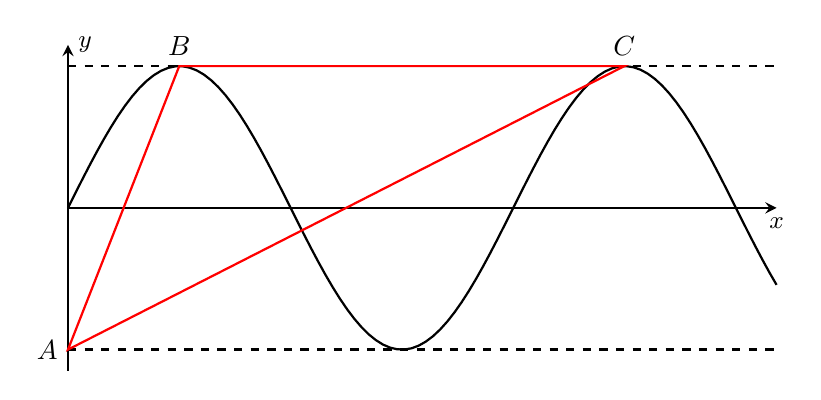
\begin{tikzpicture}[thick,>=stealth,x=1cm,y=1cm,scale=0.9] 
		\draw[->] (0,0) -- (10,0) node[below] {\small $x$};
		\draw[->] (0,-2.3) -- (0,2.3) node[right] {\small $y$};
		\draw[thick,samples=100,domain=0:10] plot(\x,{2*sin((\x)*180/pi)});
		\draw[dashed] (0,2)--(10,2);
		\draw[dashed] (0,-2)--(10,-2);
		\path (1.57,2)node[above]{$B$} (7.85,2)node[above]{$C$} (0,-2)node[left]{$A$} ;
		\draw[red] (1.57,2)--(7.85,2)--(0,-2)--cycle;
		
	\end{tikzpicture}
\end{center}
	\shortans[]{12{,}6}
	\loigiai{
		Ta có $-1\leq \sin x \leq 1 \Rightarrow-2 \leq 2 \sin x \leq 2 \Rightarrow-2 \leq f(x) \leq 2$.\\
		Xét $f(x)=2 \Leftrightarrow 2 \sin x=2 \Leftrightarrow \sin x=1 \Leftrightarrow x=\dfrac{\pi}{2}+k 2 \pi$ ($k \in \mathbb{Z}$).\\
		Với $x>0$ thì $\dfrac{\pi}{2}+k 2 \pi>0 \Leftrightarrow k>-\dfrac{1}{4}$.\\
		Mà $k \in \mathbb{Z} \Rightarrow k \in\{0;1;2;\ldots\}$.\\
		Với $k=0$ ta có $x_B=\dfrac{\pi}{2} \Rightarrow B\left(\dfrac{\pi}{2};2\right)$.\\
		Với $k=1$ ta có $x_C=\dfrac{5 \pi}{2} \Rightarrow C\left(\dfrac{5 \pi}{2};2\right)$.\\
		Ta có $A(0;-2)$.\\
		Suy ra $\mathrm{d}(A,BC)=2OA=2\cdot 2=4$.\\
		$BC=\sqrt{(2 \pi)^2+0^2}=2 \pi$.\\
		Vậy $S_{ABC}=\dfrac{1}{2} \mathrm{d}(A,BC) \cdot BC=\dfrac{1}{2} \cdot 4 \cdot 2 \pi=4 \pi \approx 12{,}6$.
	}
\end{ex}
%%%==============HetCau_EX1==============%%%
%%%==============Cau_EX2==============%%%
\begin{ex}%[Dự án C đề thi thử THPT QG 2025]%[Đỗ Chí Tâm]%[0D0V2-9]
	Trong đề kiểm tra $15$ phút môn Toán có $20$ câu trắc nghiệm. Mỗi câu trắc nghiệm có $4$ phương án trả lời, trong đó chỉ có một phương án trả lời đúng. An giải chắc chắn đúng $10$ câu, $10$ câu còn lại lựa chọn ngẫu nhiên đáp án. Biết rằng mỗi câu trả lời đúng được $0{,}5$ điểm, trả lời sai không bị trừ điểm. Xác suất để An đạt được đúng $8$ điểm là $p$. Khi đó, $100p$ bằng
	\shortans[]{1{,}6}
	\loigiai{
		Vì An chắc chắn giải đúng $10$ câu nên chắc chắn An đã được $5$ điểm.\\
		Để An được $8$ điểm thì An cần làm đúng thêm $6$ câu nữa.\\
		Chọn $6$ câu trong số $10$ câu còn lại có $\mathrm{C}_{10}^6$ cách.\\
		Mỗi câu có $4$ phương án trả lời nên xác suất đúng $1$ câu là $0{,}25$, xác suất sai $1$ câu là $0{,}75$.\\
		Vậy xác suất để An được $8$ điểm là $\mathrm{C}_{10}^6 \cdot 0{,}25^6 \cdot 0{,}75^4 \approx 0{,}016$.\\
		Vậy $100p=1{,}6$.	
		
	}
\end{ex}
%%%==============HetCau_EX3==============%%%
%%%==============Cau_EX3==============%%%
\begin{ex}%[Dự án C đề thi thử THPT QG 2025]%[Đỗ Chí Tâm]%[2D4V3-2]
	\immini[thm]{Một công ty có ý định thiết kế một logo hình vuông có độ dài nửa đường chéo bằng $4$. Biểu tượng $4$ chiếc lá (được tô màu) được tạo thành bởi các đường cong đối xứng với nhau qua tâm của hình vuông và qua các đường chéo. Một trong số các đường cong ở nửa bên phải của logo là một phần của đồ thị hàm số bậc ba dạng $y = ax^3 + bx^2 - x$ với hệ số $a<0$. Để kỷ niệm ngày thành lập $2/3$, công ty thiết kế để tỉ số diện tích được tô màu so với phần không được tô màu bằng $\dfrac{2}{3}$. Tính $2a + 2b$.
	}
	{\begin{tikzpicture}[scale=0.7, font=\footnotesize, line join=round, line cap=round,>=stealth]
			\foreach \i in {0,1,2,3}{
				\fill[pattern = north east lines,draw,smooth,rotate=90*\i] plot [domain=0:3](\x,{-(\x)*(\x-3)^2/8})--plot [domain=3:0](\x,{(\x)*(\x-3)^2/8})--cycle;
				\draw (0,0)--(90*\i:3)--(90*\i+90:3);
			}
		\end{tikzpicture}
	}
	\shortans[]{$0{,}8$}
	\loigiai
	{
		Ta có nửa đường chéo hình vuông có độ dài là $4$, cạnh hình vuông sẽ là $4\sqrt{2}$ và diện tích hình vuông là $32$, khi đó ta có được diện tích phần tô màu là $\dfrac{64}{5}$.\\
		Gọi $f(x) = ax^3 + bx^2 - x$ là hàm số bậc ba biểu diễn đường cong trên logo.\\
		Ta có $x = 4$ là nghiệm của phương trình nên $64a + 16b - 4 = 0 \Leftrightarrow 4a+b=1$.\quad (1)\\
		Do đó phương trình $f(x) = 0$ sẽ có các nghiệm là $0$, $4$.\\
		Khi đó diện tích hình phẳng $S$ giới hạn bởi các đường $y = f(x)$, trục $Ox$, đường thẳng $x = 0$, $x = 4$ là
		\begin{eqnarray*}
			S&= & \displaystyle \int \limits_{0}^{4} |ax^3+bx^2-x|\mathrm{\,d}x = -\displaystyle \int \limits_{0}^{4} (ax^3+bx^2-x)\mathrm{\,d}x\\
			&= & -\left(\dfrac{ax^4}{4}+\dfrac{bx^3}{3}-\dfrac{x^2}{2}\right)\Bigg|_0^4 = -64a-\dfrac{64}{3}b+8.
		\end{eqnarray*}
		Mà $S = \dfrac{1}{8}\cdot \dfrac{64}{5} = \dfrac{8}{5}$ nên $-64a-\dfrac{64}{3}b+8 = \dfrac{8}{5} \Leftrightarrow 64a+\dfrac{64}{3}b=\dfrac{32}{5}$.\quad (2)\\
		Từ $(1)$ và $(2)$, ta có $\heva{&4a+b=1\\&64a+\dfrac{64}{3}b=\dfrac{32}{5}} \Leftrightarrow \heva{&a = -\dfrac{1}{20}\\&b=\dfrac{9}{20}} \Rightarrow 2a+2b = \dfrac{4}{5}$.
	}
\end{ex}
%%%==============HetCau_EX4==============%%%
%%%==============Cau_EX4==============%%%
\begin{ex}%[Dự án C đề thi thử THPT QG 2025]%[Đỗ Chí Tâm]%[2D1G3-6]
	Giả sử tỉ lệ sinh của tỉnh $A$ tuân theo quy luật logistic được mô hình hóa bằng hàm số $f(t)=\dfrac{200}{1+4 \mathrm{e}^{-t}}$, $t \geq 0$, $t \in \mathbb{N}$, trong đó thời gian $t$ được tính bằng tháng. Khi đó đạo hàm $f'(t)$ sẽ biểu thị tốc độ tăng dân số của tỉnh $A$. Hỏi sau bao nhiêu tháng tốc độ tăng trưởng của dân số tỉnh $A$ là lớn nhất?
	\shortans[]{2}
	\loigiai{
		Ta có: $f'(t)=200 \cdot \dfrac{4 \mathrm{e}^{-t}}{\left(1+4 \mathrm{e}^{-t}\right)^2}=\dfrac{800 \mathrm{e}^{-t}}{\left(1+4 \mathrm{e}^{-t}\right)^2}$
		\begin{eqnarray*}
			f^{\prime \prime}(t)&=&800 \cdot \dfrac{-\mathrm{e}^{-t}\left(1+4 \mathrm{e}^{-t}\right)^2-\mathrm{e}^{-t} \cdot 2 \cdot\left(-4 \mathrm{e}^{-t}\right)\left(1+4 \mathrm{e}^{-t}\right)}{\left(1+4 \mathrm{e}^{-t}\right)^4}\\
			&=&800 \cdot \dfrac{4\left(\mathrm{e}^{-t}\right)^2-\mathrm{e}^{-t}}{\left(1+4 \mathrm{e}^{-t}\right)^2}\\
			&=&\dfrac{800 \mathrm{e}^{-t}}{\left(1+4 \mathrm{e}^{-t}\right)^3}\left(4 \mathrm{e}^{-t}-1\right).
		\end{eqnarray*}
		$$f^{\prime \prime}(t)=0 \Leftrightarrow 4 \mathrm{e}^{-t}-1=0 \Leftrightarrow \mathrm{e}^{-t}=\dfrac{1}{4} \Leftrightarrow t=\ln 4.$$
		Bảng biến thiên
		\begin{center}
			
\begin{tikzpicture}[font=\normalsize,t style/.style={style=solid}]
				\tkzTabInit[nocadre=true,lgt=1.2,espcl=2.5,deltacl=0.5]
				{$t$ /0.75, $f^{\prime\prime}(t)$/0.75, $f'(t)$/2}
				{$ 0 $,$\ln4 $,$+\infty $}
				\tkzTabLine{,+,0,-,}  % z, t, d;
				\tkzTabVar{-/$32$,+/$50$,-/$0$} %+ hoac-
			\end{tikzpicture}
		\end{center}
		Từ bảng biến thiên ta thấy giá trị lớn nhất của $f'(t)$ là $50$ xảy ra tại $t=\ln 4$.\\
		Vậy sau khoảng $2$ tháng thì tốc độ tăng trưởng dân số của tỉnh $A$ là lớn nhất.
		
	}
\end{ex}
%%%==============HetCau_EX4==============%%%
%%%==============Cau_EX5==============%%%
\begin{ex}%[Dự án C đề thi thử THPT QG 2025]%[Đỗ Chí Tâm]%[2D1G3-6]
	\immini{Một máy bay trình diễn có đường bay gắn với hệ trục $Oxy$ được mô phỏng như hình vẽ, trục $Ox$ gắn với mặt đất. Đường bay có dạng là một phần của đồ thị của hàm phân thức bậc hai trên bậc nhất $y=f(x)$ có đường tiệm cận đứng $x=2$. Điểm $G$ là giao điểm của đường tiệm cận xiên của đồ thị hàm số $y=f(x)$ và trục $Ox$ được gọi là điểm giới hạn. Biết rằng máy bay xuất phát tại vị trí $A$ cách gốc tọa độ $O$ một khoảng $2{,}5$ đơn vị và máy bay khi ở vị trí cao nhất cách điểm xuất phát $1{,}5$ đơn vị theo phương song song với trục $Ox$ và cách mặt đất $4{,}5$ đơn vị. Vị trí máy bay tiếp đất cách điểm giới hạn một khoảng bằng bao nhiêu?}
	{\begin{tikzpicture}[scale=0.5,>=stealth, font=\footnotesize, line join=round, line cap=round]
			\draw[->] (-0.5,0)--(11,0)node[below]{$x$};
			\draw[->] (0,-1.8)--(0,9)node[right]{$y$};
			\draw[samples=100,domain=2.4:10.3] plot (\x,{(-(\x)^2+12.5*(\x)-25)/((\x)-2)});
			\draw[samples=100,domain=1.6:10.6] plot (\x,{(-(\x)+10.5)});
			\draw(2,-1.8)--(2,9);
			\draw(0,0)node[below right]{$O$};
			\draw (4,4.5)circle (1.3pt)node[above]{$B$}(2.5,0)circle (1.3pt)node[below right]{$A$}(10,0)circle (1.3pt)node[below]{$C$}(10.5,0)circle (1.3pt)node[above]{$G$};%--(-2,4)--(0,4)node[right]{$4$}
		%	(2,0)node[above]{$2$}--(2,-4)--(0,-4)node[left]{$-4$};
	\end{tikzpicture}}
	\shortans[]{0{,}5}
	\loigiai{
		Hàm số bậc hai trên bậc nhất có dạng $y=f(x)=\dfrac{ax^2+bx+c}{x-2}$.\\
		Theo giả thiết ta có $A(2{,}5;0)$, $B(4; 4{,}5)$.\\
		Vì $A$, $B$ thuộc đồ thị hàm số nên $\heva{&6{,}25a+2{,}5b+c=0 \\& 16a+4b+c=9.}$\\
		Ta có
		$ f'(x)=\dfrac{ax^2-4ax-2b-c}{(x-2)^2}$.\\
		$f'\left(x_B\right)=0 \Rightarrow \dfrac{a \cdot 4^2-4a \cdot 4-2b-c}{(4-2)^2}=0 \Rightarrow 2b+c=0$.\\
		Từ $(1)$ và $(2)$ suy ra $a=-1$, $b=12{,}5$, $c=-25$.\\
		Khi đó $f(x)=\dfrac{-x^2+12{,}5x-25}{x-2}=-x+10{,}5-\dfrac{4}{x-2}$.\\
		\[\lim\limits_{x \rightarrow+\infty}[f(x)-(-x+10{,}5)]=\lim \limits_{x \rightarrow+\infty}\left(-x+10{,}5-\dfrac{4}{x-2}+x-10,5\right)=\lim \limits_{x \rightarrow+\infty} \dfrac{-4}{x-2}=0.\]		
		Vậy $y=-x+10{,}5$ là tiệm cận xiên của đồ thị hàm số.\\
		Tọa độ giao điểm $G$ là nghiệm của hệ phương trình $\heva{&y=-x+10{,}5 \\& y=0} \Leftrightarrow\heva{&x=10{,}5 \\& y=0} \Rightarrow G(10{,}5 0)$.\\
		Tương tự ta tìm được $A(2{,}5;0)$, $C(10;0)$.\\
		$CG=x_G-x_C=10{,}5-10=0{,}5$.\\
		Vậy vị trí máy bay tiếp đất cách điểm giới hạn một khoảng $0{,}5$ đơn vị.	
	}
\end{ex}
%%%==============HetCau_EX5==============%%%
%%%==============Cau_EX6==============%%%
\begin{ex}%[Dự án C đề thi thử THPT QG 2025]%[Đỗ Chí Tâm]%[0H5C2-6]
	\immini{Có ba lực cùng tác động vào một cái bàn như hình vẽ. Trong đó hai lực $\overrightarrow{F}_1, \overrightarrow{F}_2$ có giá nằm trên mặt phẳng chứa mặt bàn, tạo với nhau một góc $110^{\circ}$ và có độ lớn lần lượt là $9$ N, $4$ N, lực $\overrightarrow{F}_3$ vuông góc với mặt bàn và có độ lớn $7$ N. Độ lớn hợp lực của ba lực trên là $a$ (N), tìm giá trị của $a$ (\textit{kết quả làm tròn đến hàng đơn vị})}{\includegraphics[scale=0.4]{images/TT-THPT-SGD-HaTinh-NH24-25}}
	\shortans{11}
	\loigiai{
		Ta có \begin{eqnarray*}
			\left|\overrightarrow{F}_1+\overrightarrow{F}_2+\overrightarrow{F}_3\right|&=&\sqrt{\left(\overrightarrow{F}_1+\overrightarrow{F}_2+\overrightarrow{F}_3\right)} \\
			& =&\sqrt{F_1^2+F_2^2+F_3^2+2 \overrightarrow{F}_1 \overrightarrow{F}_2+2 \overrightarrow{F}_2 \overrightarrow{F}_3+2 \overrightarrow{F}_3 \overrightarrow{F}_1} \\
			& =&\sqrt{F_1^2+F_2^2+F_3^2+2 F_1 F_2 \cos 110^{\circ}+2 F_2 F_3 \cos 90^{\circ}+2 F_1 F_3 \cos 90^{\circ}} \\
			& =&\sqrt{9^2+4^2+7^2+2 \cdot 9 \cdot 4 \cdot \cos 10^{\circ}+2 \cdot 4 \cdot 7 \cdot 0+2 \cdot 9 \cdot 7 \cdot 0} \approx 11\,(\text{N}).
		\end{eqnarray*} 
}
\end{ex}
 \Closesolutionfile{ans}
\inputansbox{6,4,3}{ans/TT-THPT-SGD-HaTinh-NH24-25}